\section{Game Design}


Figure \ref{fig:player-screenshots} illustrates what the game
interface may look like for players one and two at some point in the
game\footnote{While the game is fully playable, the interface is still
  a prototype in which everything is represented by differently
  colored blocks.}. The red block is player one's avatar, the green
block player two's avatar. The purple block is the ball, which needs
to be pushed to the goal represented by the orange block. The white
and gray blocks are portals. Portals come in pairs -- if the ball or
player enter one portal, they exit through another one --- and
connect different areas of one player's environment or link one
player's environment with the other's. The white portals are open to
both the ball and the player; the gray portals can only be used by the
ball.

%% Commented this out because we already say something similar in the
%% previous section. KS
%% The goal for this game was to have two players communicate and
%% collaborate with each other in order to push a block to a certain
%% location on the screen, the goal. The game consists of two different
%% screens of the same size: one that is only visible to player one and
%% another that is only visible to player two. Figure
%% \ref{fig:player-screenshots} shows an example screen for player one
%% and two.

\begin{figure}
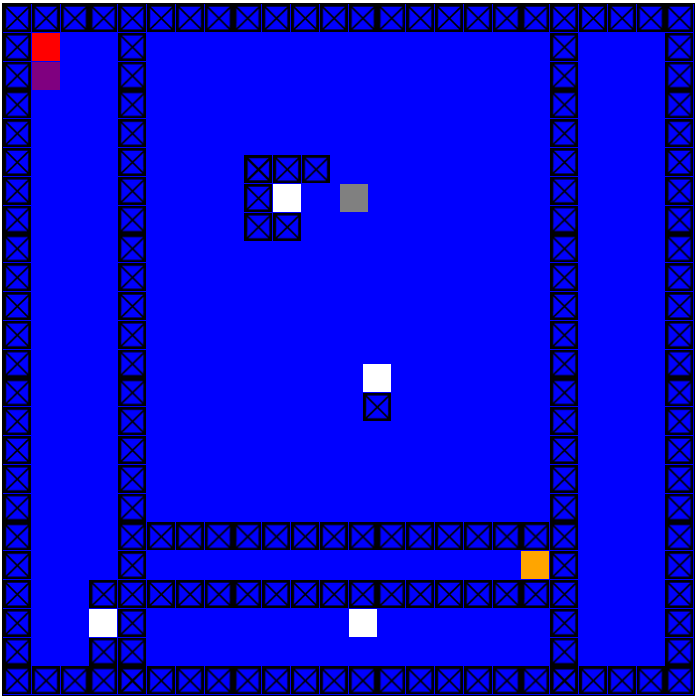
\includegraphics[scale=0.27]{playerview1.png} 
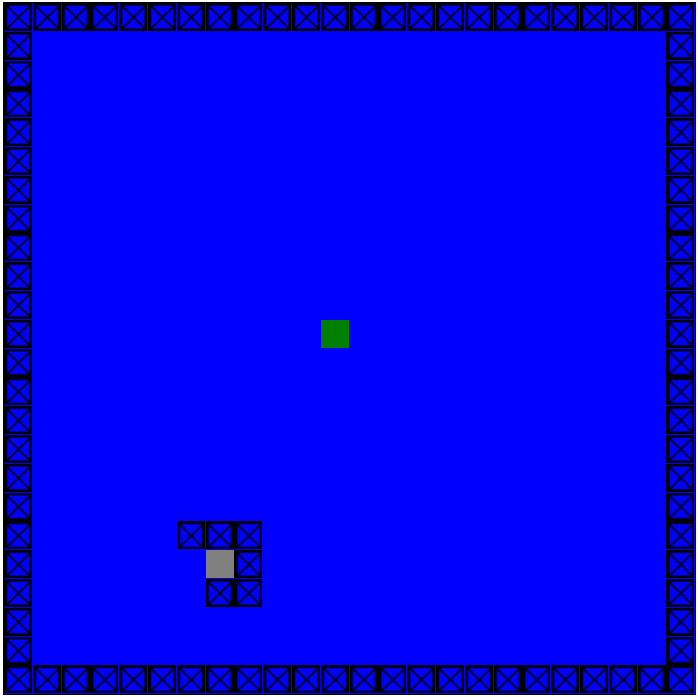
\includegraphics[scale=0.27]{playerview2.png}
\caption{Sample game screens for players one and two.\todo{let's get
    screenshots that show the chat area; I will try to fix css today
    or tomorrow - KS}}
\label{fig:player-screenshots}
\end{figure}

% what players see and do; moving the ball

The players can move their avatars using the arrow keys on their
keyboard. When they push the ball, it starts moving in the direction
of the push and only stops when it collides with an obstacle. If the
ball cannot move in the direction of the push (e.g. because there is
an obstacle), it (randomly) picks a direction that is free of
obstacles to move to, as illustrated in Figure
\ref{fig:pushing-against-wall}. This behavior makes sure that the ball
does not get trapped too easily.

\begin{figure}
\todo{Add images.}
\caption{Behavior of the ball.}
\label{fig:pushing-against-wall}
\end{figure}

% placing of blocks

Pressing the \todo{which?} key allows players to place an obstacle
into their partner's environment at the position that corresponds to
the player's current location. Each player can only place three blocks
on their partner's screen at a time. When the fourth block is placed,
the block that was placed first is deleted, as shown in Figure
\ref{fig:dropping-blocks}.

\begin{figure}
\hspace*{\fill}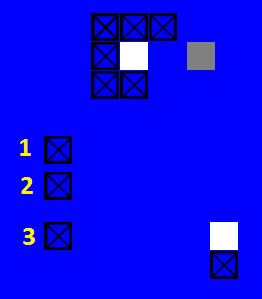
\includegraphics[width=0.45\columnwidth]{blocksplaced1-cropped.png}
\hspace*{\fill}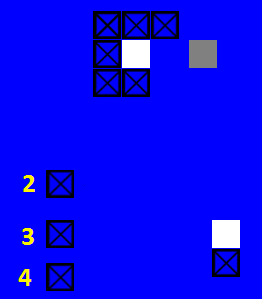
\includegraphics[width=0.45\columnwidth]{blocksplaced2-cropped.png}\hspace*{\fill}
\caption{
This figure illustrates what happens when more than three
blocks are placed by player two. The picture on the left shows a
screenshot with three blocks already placed in a line in the near the
middle of the screen. The numbers next to the blocks correspond to
when they were placed. For example, the block with the one next to it
was the first block placed and so on. The picture on the right shows
what happens when another block is placed after three are already
placed. The block that gets deleted was the first of all the blocks
placed in the left picture.}\label{fig:dropping-blocks}
\end{figure}

The players cannot place obstacles into their own environments, but
since obstacles are the only way to stop a ball that is moving they
have to collaborate to control the balls movements. 
The environments are designed to force the players to work together
and communicate with each other.

\todo{This is how far I got; still need to finish the rest, but
  checking in now; because I have to go to the office. KS}

% visibility of screens - and chatting

On each screen is a maze created from various obstacles that must be
overcome in order to push the block to the goal block. The obstacles
can be overcome by the strategic placement of blocks that each player
can place on their partner's screen. However, since each players'
screen is invisible to their partner, players must provide typed
instructions leading to the precise location that a block needs to be
placed. Players must interpret the directions and move to the position
they believe that their partner is describing. Players can then place
a block on their partner's screen at the same position that they
currently are on their own screen. 

% kinds of obstacles
